\section{实际算例}

以下为地铁隧道的一个切面数据:
\begin{table}[!htbp]
    \centering
    \begin{tabular}{ccc} \hline
        x & y & h \\ \hline
        221483.4277 & 217541.3367 & 480.7289 \\
        221483.4384 & 217541.3517 & 480.7276 \\
        \ldots & \ldots & \ldots \\
        221484.7543 & 217544.2667 & 485.0110 \\ \hline
    \end{tabular}
    \caption{切面数据}
\end{table}

其$xy$平面散点图如下:
\begin{figure}[!htbp]
    \centering
    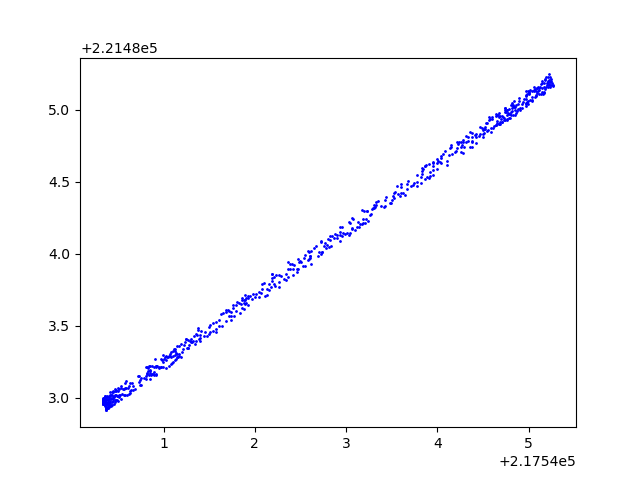
\includegraphics[width =\textwidth]{01.png}
    \caption{$xy$平面散点图}
\end{figure}

使用特征根方法进行直线拟合, 见\eqref{evfit}于\pageref{evfit}
\begin{table}[!htbp]
    \centering
    \begin{tabular}{cl} \hline 
        a & 0.908938 \\ 
        b & -0.416912 \\
        c & 0.004054 \\
        d & -110620.998330 \\ \hline
    \end{tabular}
    \caption{直线参数}
\end{table}

直线方程为 $0.908938x-0.416912y+0.004054h-110620.998330=0$

原始数据投影至拟合平面, 其坐标为:
\begin{table}[!htbp]
    \centering
    \begin{tabular}{ccc} \hline
        x & y & h \\ \hline
        221483.4194 & 217541.3404 & 480.7288 \\
        221483.4270 & 217541.3569 & 480.7275 \\
        221483.3804 & 217541.2555 & 480.7460 \\
        \ldots & \ldots & \ldots \\
        221484.7311 & 217544.2419 & 485.0347 \\
        221484.7446 & 217544.2711 & 485.0109 \\ \hline
    \end{tabular}
    \caption{投影点数据}
\end{table}

再将投影点数据转换为平面坐标:
\begin{table}[!htbp]
    \centering
    \begin{tabular}{ccc} \hline
        x & y \\ \hline
        -2.84722883 & -1.45261677 \\
        -2.84873517 & -1.43453659 \\
        -2.8290454 & -1.54593576 \\
        \ldots & \ldots \\
        1.42457227 & 1.77706625 \\
        1.40046748 & 1.80901189 \\ \hline
    \end{tabular}
    \caption{平面$xy$数据}
\end{table}

其可视化效果如下:
\begin{figure}[!htbp]
    \centering
    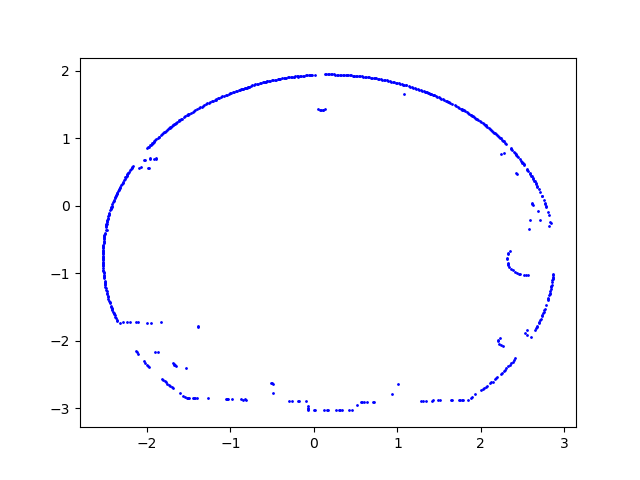
\includegraphics[width =\textwidth]{02.png}
    \caption{投影后$xy$平面散点图}
\end{figure}